\subsection{Implementation}

To demonstrate the power of the network-side adaption, we decided to adapt a legacy-device which has been in real-world use for some time.
We decided on the ''Treetalker'' platform\footnote{\url{https://www.nature4shop.com/}}, which is a product for distributed tree-health monitoring.
This platform has been in use in many areas in the world for example in Moscow city with 250 TreeTalkers or a cooperation with the Peking University. \footnote{https://www.nature4shop.com/our-vision/}

The platform vendor sells both the sensor-devices (henceforth simply called \textit{Treetalker}), as well as a basestation (henceforth called \textit{TTCloud}), which can be used to aggregate data via LoRa and upload it to a proprietary cloud-storage provider via GSM.
The ''Treetalker''-platform is proprietary, and does not give buyers access to the device firmware.

For our project, we aimed to replace the static \textit{TTCloud}, with a more versatile gateway, to allow for dynamic reconfiguration of all \textit{Treetalkers}.
We call the resulting system \ttt.

\todo{Mehrere Revisionen}

\subsubsection{TreeTalker Network}
\label{sec:implementation:treetalker:current}

Figure \ref{fig:tt-current} shows the basic architecture of a small TreeTalker-network, as intended by the vendor.

\begin{figure}
    \centering
    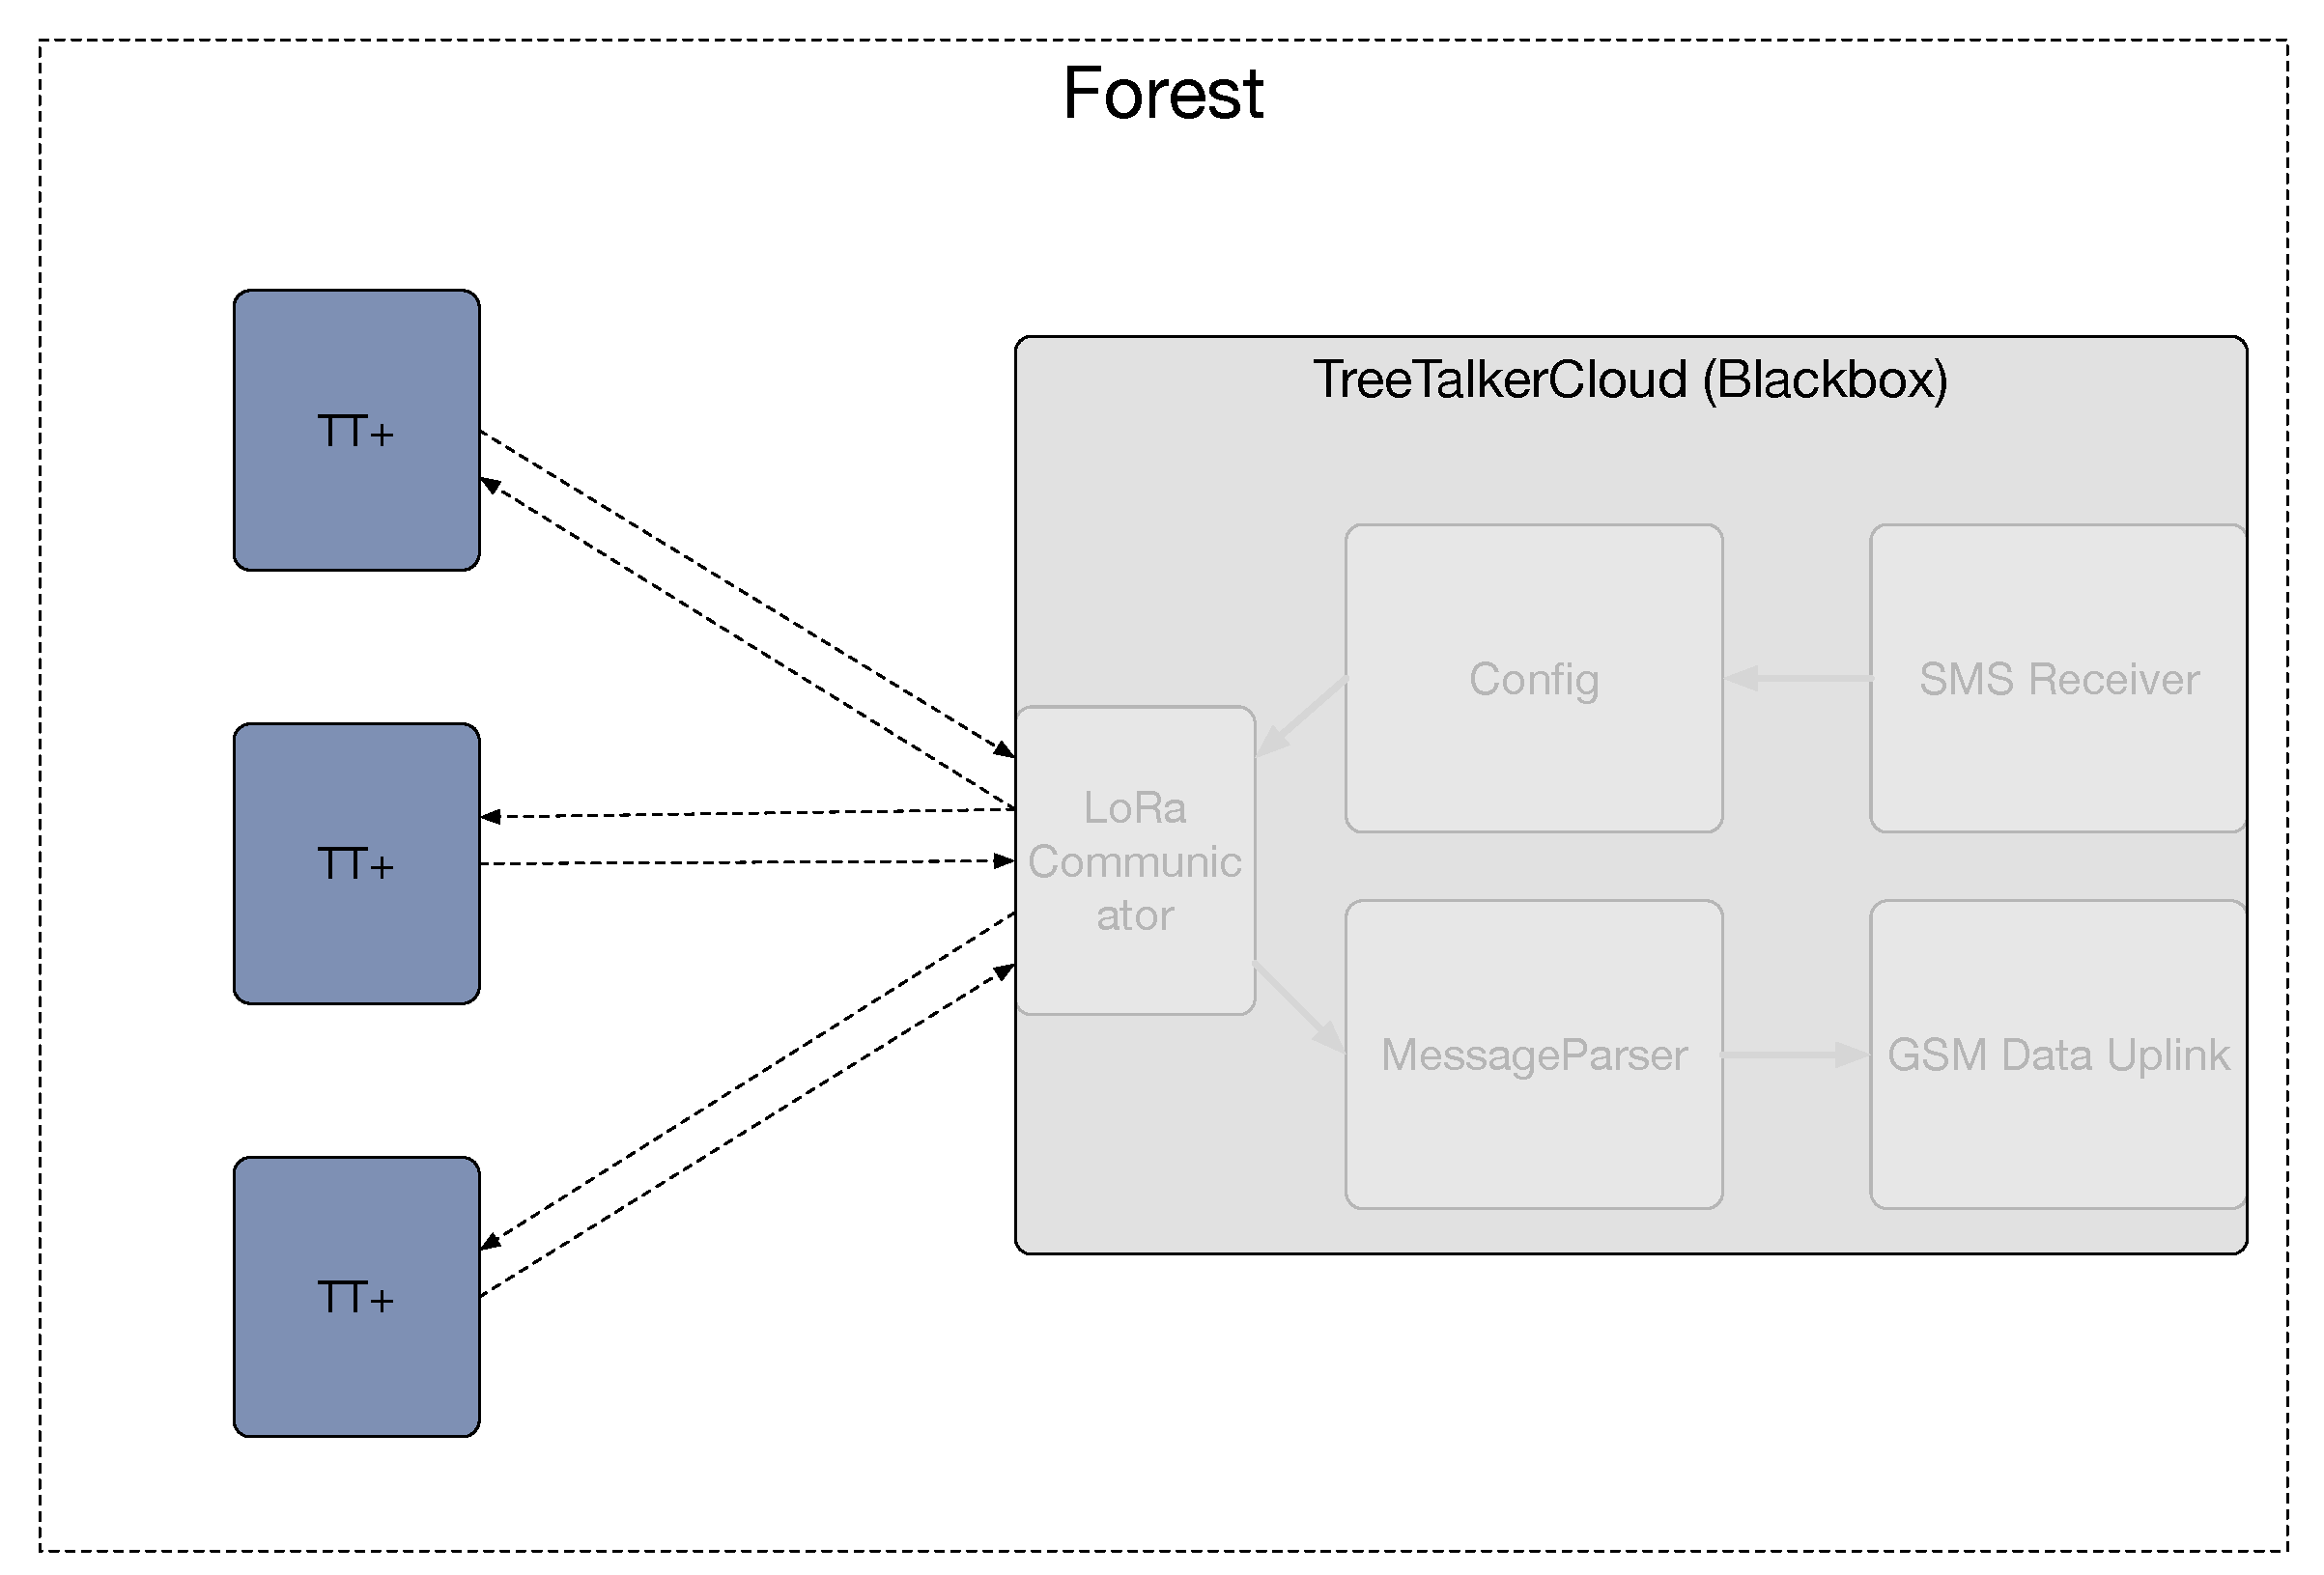
\includegraphics[width=.8\linewidth]{figures/TT_current.pdf}
    \caption{Current working schema of TT with the TTCloud}
    \label{fig:tt-current}
\end{figure}

A TTCloud can have an arbitrary number of associated Treetalkers, while a Treetalker is always associated to exactly one TTCloud.
Communication between the TTCloud and its sensor-stations is a call-response-protocol, initiated by the TreeTalker.
For a in-depth explanation of the communication protocol, see section \ref{sec:implementation:treetalker:protocol}.

While the TTCloud is a black box and thus its inner workings are unknown to us, we can make an educated guess as to its (software-)components.
The TTCloud, and its associated Treetalkers, can be configured via text-message, also, collected data is sent to the cloud-backend via a mobile data connection\footnote{the deployer needs to provide their own SIM-card with a Text-/Data-Plan}

\subsubsection{Communication Protocol}
\label{sec:implementation:treetalker:protocol}

While LoRa-alliance certified hardware provides a dedicated network-layer-protocol, called \textit{LoRa-WAN} which deals with collisions, addressing, and other issues resulting from the shared-medium characteristic of LoRa, the \textit{Treetalker}-vendor decided to forgo this higher-level protocol in favor of using the LoRa-PHY-layer directly.

For this reason, communication with each \textit{Treetalker} needs to be scheduled manually in such a way that avoids collisions.

In order to replace the \textit{TTCloud} with our own gateway, we performed a blackbox-analysis of \textit{Treetalker's} behaviour and network communications, to understand the communication protocol.

With the insights gathered by our analysis we were able to fully replace and improve the gateway functionality, which allowed us to bring the concept of \textit{mechanism-migration} to the treetalker-network.

All in all, we discovered 4 kinds of command and control packets as well as a number of different data packets with which the \textit{Treetalker} communicates its measurement data to the gateway.

\paragraph{Command and Control}

After initialisation, each \textit{Treetalker} performs a two-way handshake with the gateway, by first sending a \texttt{TTHelo}-packet and waiting for a \texttt{TTCloudHelo}-response.\footnote{Since the protocol specification is not available, all packet- and field-names were chosen by us ans might differ from ''official'' sources.}

\begin{figure}
    \centering
    \begin{bytefield}[bitwidth=1.1em]{14}
      \bitheader{0-13}\\
      \begin{rightwordgroup}{\texttt{TTHelo}}
        \bitbox{4}{Recv}
        \bitbox{4}{Snd}
        \bitbox{1}{T}
        \bitbox{1}{\#}
      \end{rightwordgroup} \\
      \begin{rightwordgroup}{\texttt{TTCloudHelo}}
        \bitbox{4}{Recv}
        \bitbox{4}{Snd}
        \bitbox{1}{T}
        \bitbox{1}{C}
        \bitbox{4}{Time}
      \end{rightwordgroup}
    \end{bytefield}
    \caption{HELO-Packets}
    \label{fig:tthelo}
\end{figure}

The packet-formats can be seen in figure \ref{fig:tthelo}.
All packets share the same first 3 fields \texttt{Recv}, which is the receiver address, \texttt{Snd}, the sender address, and \texttt{T} which is the \textit{packet type}, which is a unique value for each kind of packet.

The \texttt{TTHelo}-packet also includes a field \texttt{\#}, which starts at 0 and counts up for each sent HELO-packet that didn't produce a response.
The \texttt{TTCloudHelo}-packet hast a field \texttt{C}, or ''command'' which appears to depend on the \textit{TTCloud}-revision, but does not seem to produce any differing behaviour in \textit{Treetalkers}.
Furthermore, as part of its HELO-packet the gateway send its current system time (as a UNIX-style timestamp) in the \texttt{Time} field.
This allows the \textit{Treetalker} to initialise its own internal clock.

Once it receives a \texttt{TTCloudHelo}-packet, the \textit{Treetalker} will attach itself to the gateway and will start collecting measurement data.

There are a further 2 command-type packets with which the gateway can configure \textit{Treetalker} behaviour, these can be seen in figures \ref{fig:ttcommand}.

\begin{figure}
    \centering
    \begin{bytefield}[bitwidth=1.1em]{22}
      \bitheader{0-21}\\
      \begin{rightwordgroup}{\texttt{TTCommand1}}
        \bitbox{4}{Recv}
        \bitbox{4}{Snd}
        \bitbox{1}{T}
        \bitbox{1}{C}
        \bitbox{4}{Time}
        \bitbox{4}{Sleep}
        \bitbox{2}{ht}
        \bitbox{1}{l}
        \bitbox{1}{s}
      \end{rightwordgroup} \\
      \begin{rightwordgroup}{\texttt{TTCommand2}}
        \bitbox{4}{Recv}
        \bitbox{4}{Snd}
        \bitbox{1}{T}
        \bitbox{1}{C}
        \bitbox{4}{Time}
        \bitbox{1}{i}
        \bitbox{1}{g}
      \end{rightwordgroup}
    \end{bytefield}
    \caption{Command Packets}
    \label{fig:ttcommand}
\end{figure}

\begin{figure}
    \centering
    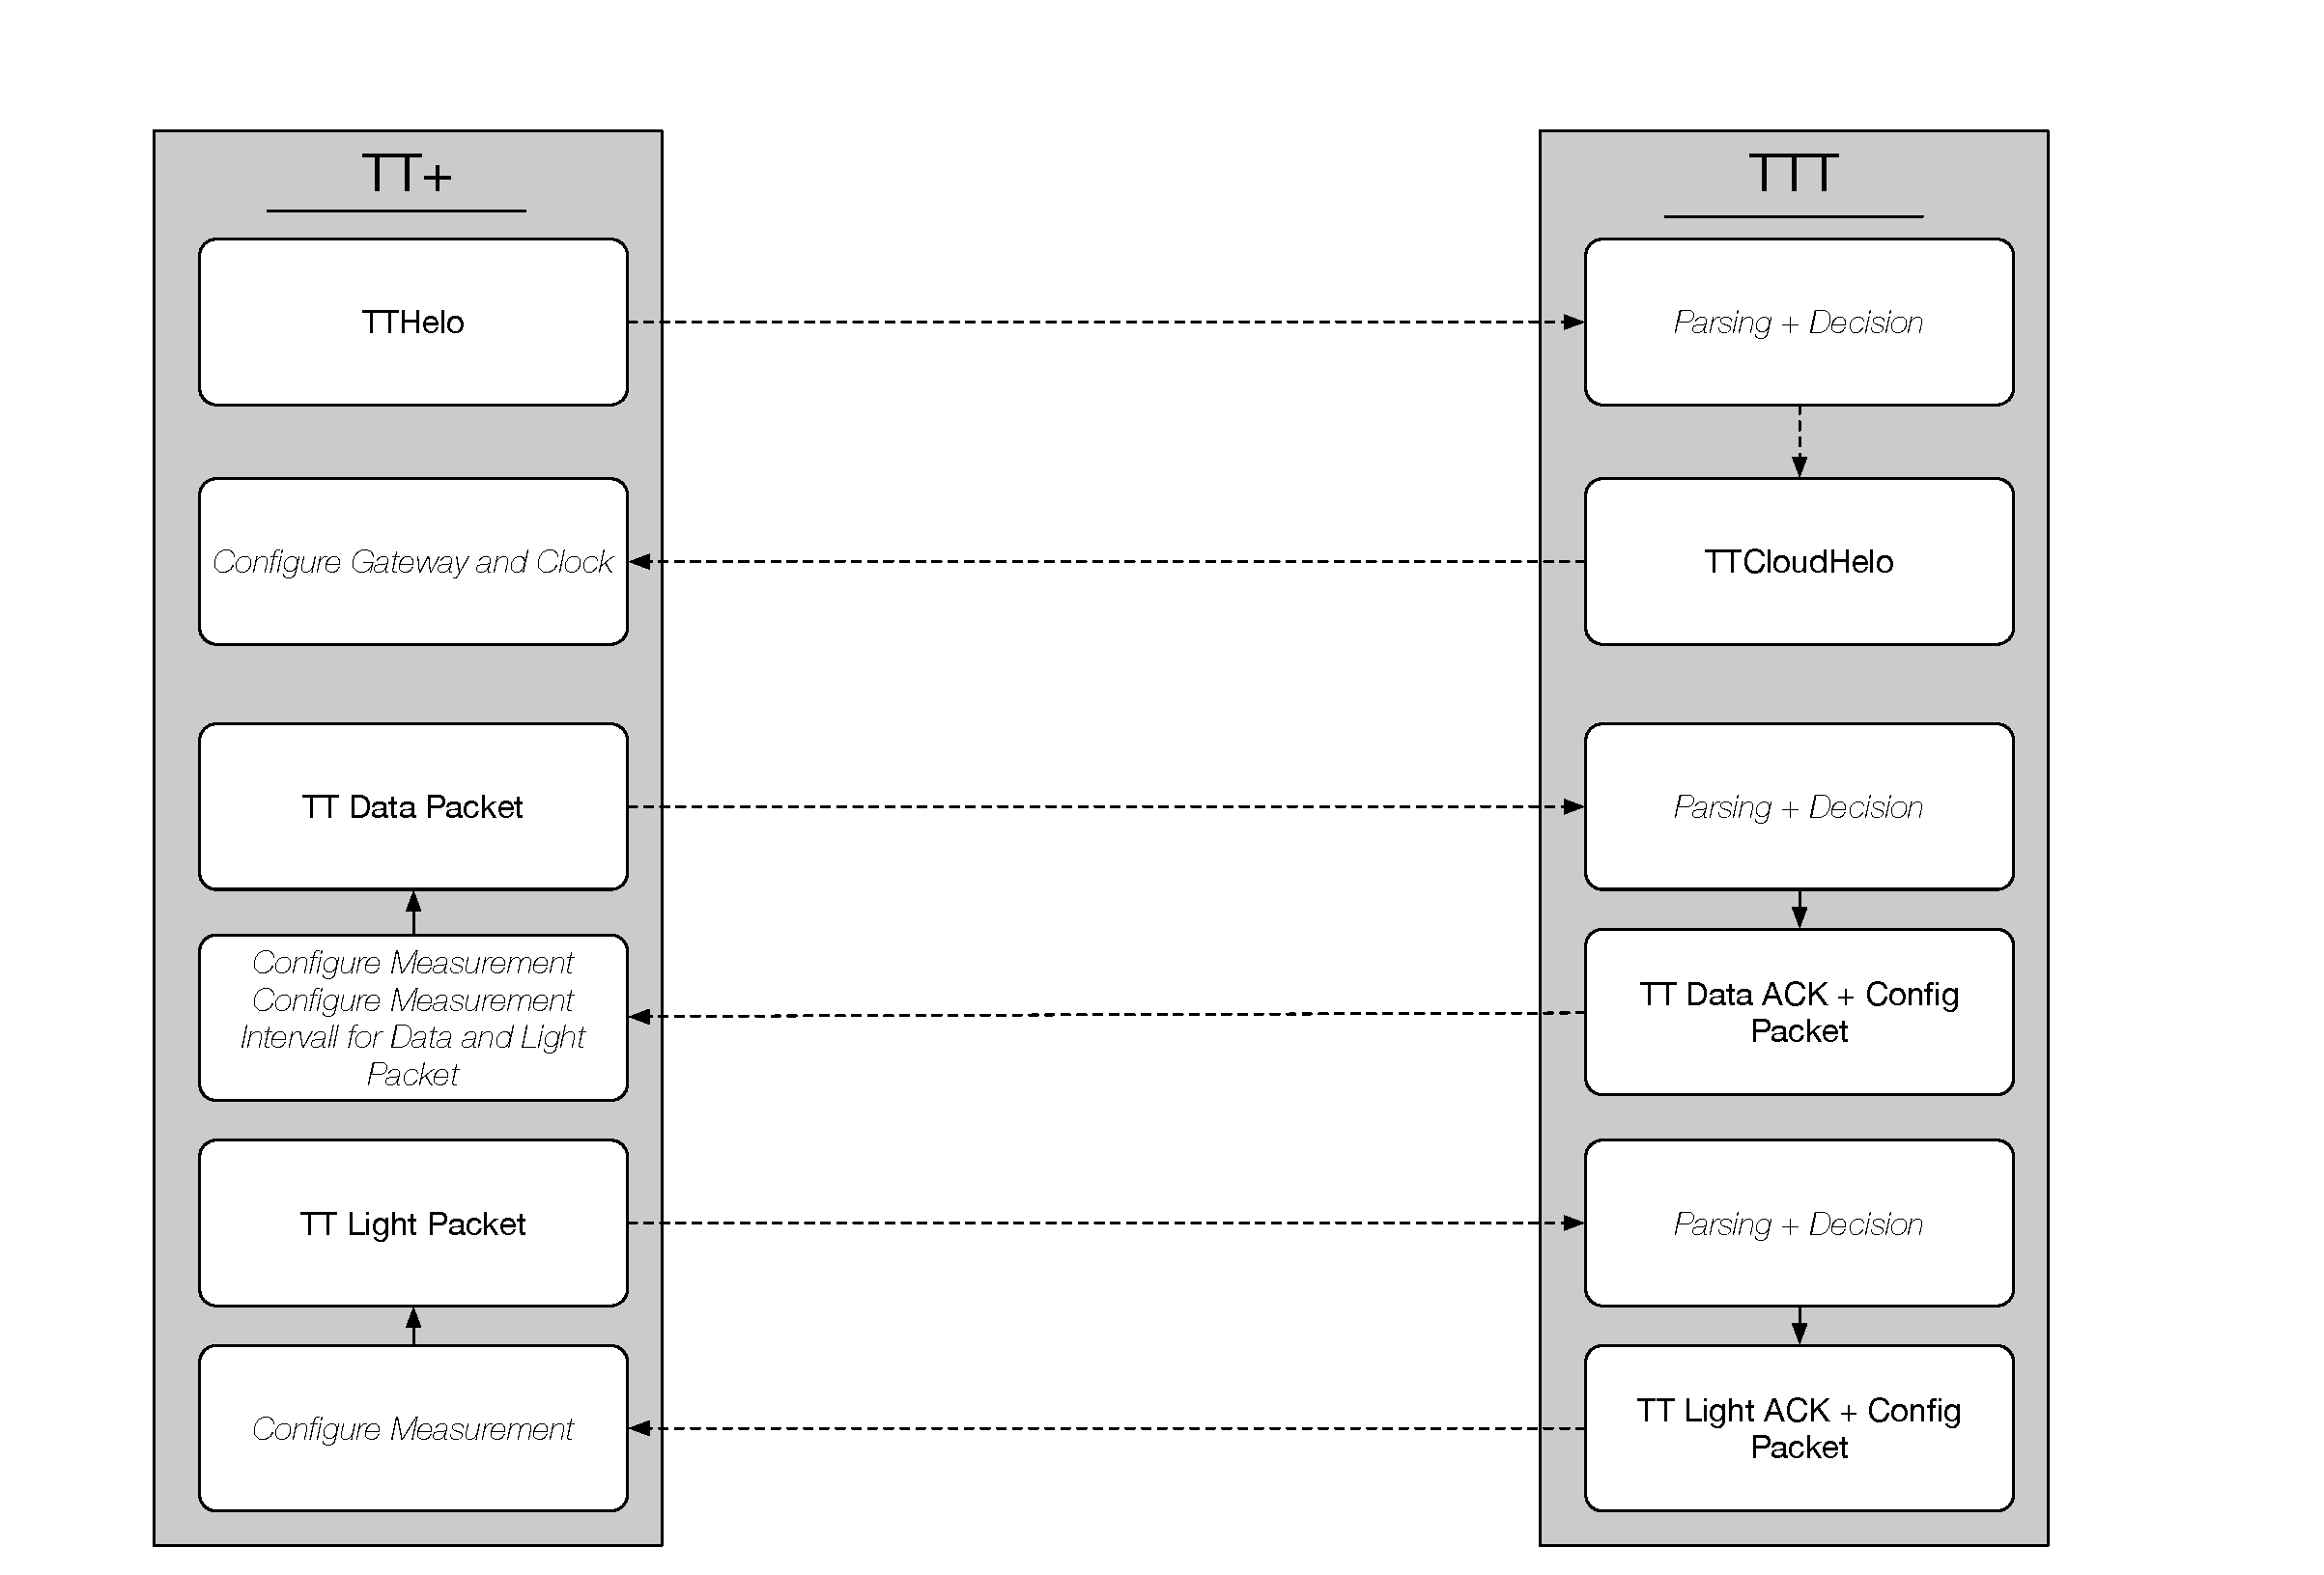
\includegraphics[width=.8\linewidth]{figures/TT_protocol_flowchart.pdf}
    \caption{Protocol flowchart for TT+ with TTCloud}
    \label{fig:tt-protocol}
\end{figure}

The \texttt{TTCommand1} contains 4 fields, with which the \textit{Treetalker's} behaviour can be influenced.
\texttt{Sleep} is the time that the device will sit idle in between measurements (defaults to 1 hour).
\texttt{ht} is the \textit{Heating Time}, that is how long the \textit{Treetalker} will run its internal heater before taking the second set of heat-probe measurments.
Lastly, we have \texttt{l} and \texttt{s}, the time slot length and assigned time slot respectively.
These values govern the time that the device will wait between measurements and sending measurement data, it appears that these two values are simply multiplied to get the time-to-wait before transmitting.

In normal operation, with a vendor-supplied gateway, the sleep- and heat-time are user-configurable, but fixed, and the same for all \textit{Treetalkers} attached to the gateway.
The time slot length will also be the same for all nodes, while the gateway will assign each \textit{Treetalker} a unique time slot.
Again, this is necessary due to the vendor's refusal to use the \textit{LoRaWAN}-protocol, which includes a mechanism for collision-avoidance, but since the \textit{Treetalker}-system uses the raw \textit{LoRaPHY}-layer, the gateway needs to schedule transmission manually.
For this reason, there is also no way for a \textit{Treetalker}-network to coexist with other LoRa-networks in the same area, since collisions would be plenty and unrecoverable.

The other control message, \texttt{TTCommand2}, provides merely configuration for the built-in light sensors, and is largely irrelevant for our usecase.

\paragraph{Data}

As there are two kinds of command, there are also two kinds of data-packets.
The exact makeup of these packets is not relevant, but they contain the measurement data from the \textit{Treetalkers} sensors, which are the following:

\begin{itemize}
    \item 2 temperature probes (named ''reference'' and ''heat'') which are inserted into drill-holes in the tree's trunk and measure heat-transfer inside the tress, which can be used to calculate sap-flow.
    \item A growth-sensor, which is affixed to the tree's outside using fixed-length standoffs.
    It measures its distance to the bark to track the growth of the tree's circumference over long times.
    \item Battery Voltage
    \item Air humidity \& Temperature
    \item Three-axis accelerometer
    \item Two light sensors, operating at slightly different wavelengths
\end{itemize}

This data is used as the basis for the Anomaly- \& Error-Detection which we will further elaborate on in section \ref{sec:implementation:treetalker:error-detection}.

\subsubsection{Findings / Behaviour of the TTT}
To analyze the \textit{TreeTalkers}, we recorded the data stream on the Lora network between the official gateway and a small cluster of \textit{Treetalkers} over a period of several days. After some passive observations, we also adjusted the configuration parameters of the official gateway to provoke certain reactions in the \textit{Treetalkers} and thus better understand the proprietary protocol.

In the process, we noticed a few peculiarities:

\paragraph{Stack}
In the event of faulty transmissions without a subsequent TTCommand packet as a response from the official gateway, the packets are retransmitted several times from the \textit{Treetalker}. If after five attempts no TTCommand has been received, the packet is stored in a non-volatile memory on the \textit{Treetalkers}. All subsequent packets were then also stored temporarily while no retransmission was attempted anymore.

In our tests, after a power cycle of the \textit{Treetalkers}, all cached packets were subsequently transmitted to the gateway at maximum transmission speed, provided that only a single \textit{Treetalker} was connected to the gateway.

\paragraph{Rate Limiter}
Due to an error in the data transmission (probably a congestion of the radio medium), data packets were written to the buffer over a period of 24 hours. After the end of the incident, the \textit{Treetalker} transmitted data to the gateway again, but not all at once, as observed after a power cycle, but at the same interval as newly added packets. This delayed the data received by the gateway by about 24 hours on the time axis, presumably the buffer was processed according to the principle "first in, first out". Our assumption is that a rate limiter was activated. Unfortunately, due to the lack of availability of the source code, we could not find out exactly what caused this behavior.

\paragraph{Bricked}
In one of our tests, a \textit{Treetalker} was rendered inoperable by setting the measurement duration in the gateway operation system to be longer than the general measurement interval. This caused all \textit{Treetalkers} connected to the gateway to be in a continuous reboot loop. Apparently, TTCommand commands transmitted via the gateway are not evaluated for their correctness. 

\paragraph{Low Power}
We could observe that the \textit{Treetalkers} monitor the battery power, but do not pay any consideration to this value. Despite summer sun and maximum exposure of the solar cells, the energy consumption was so high that we regularly ran out of power. 

\subsubsection{Anomaly- \& Error-Detection}
\begin{figure}
    \centering
    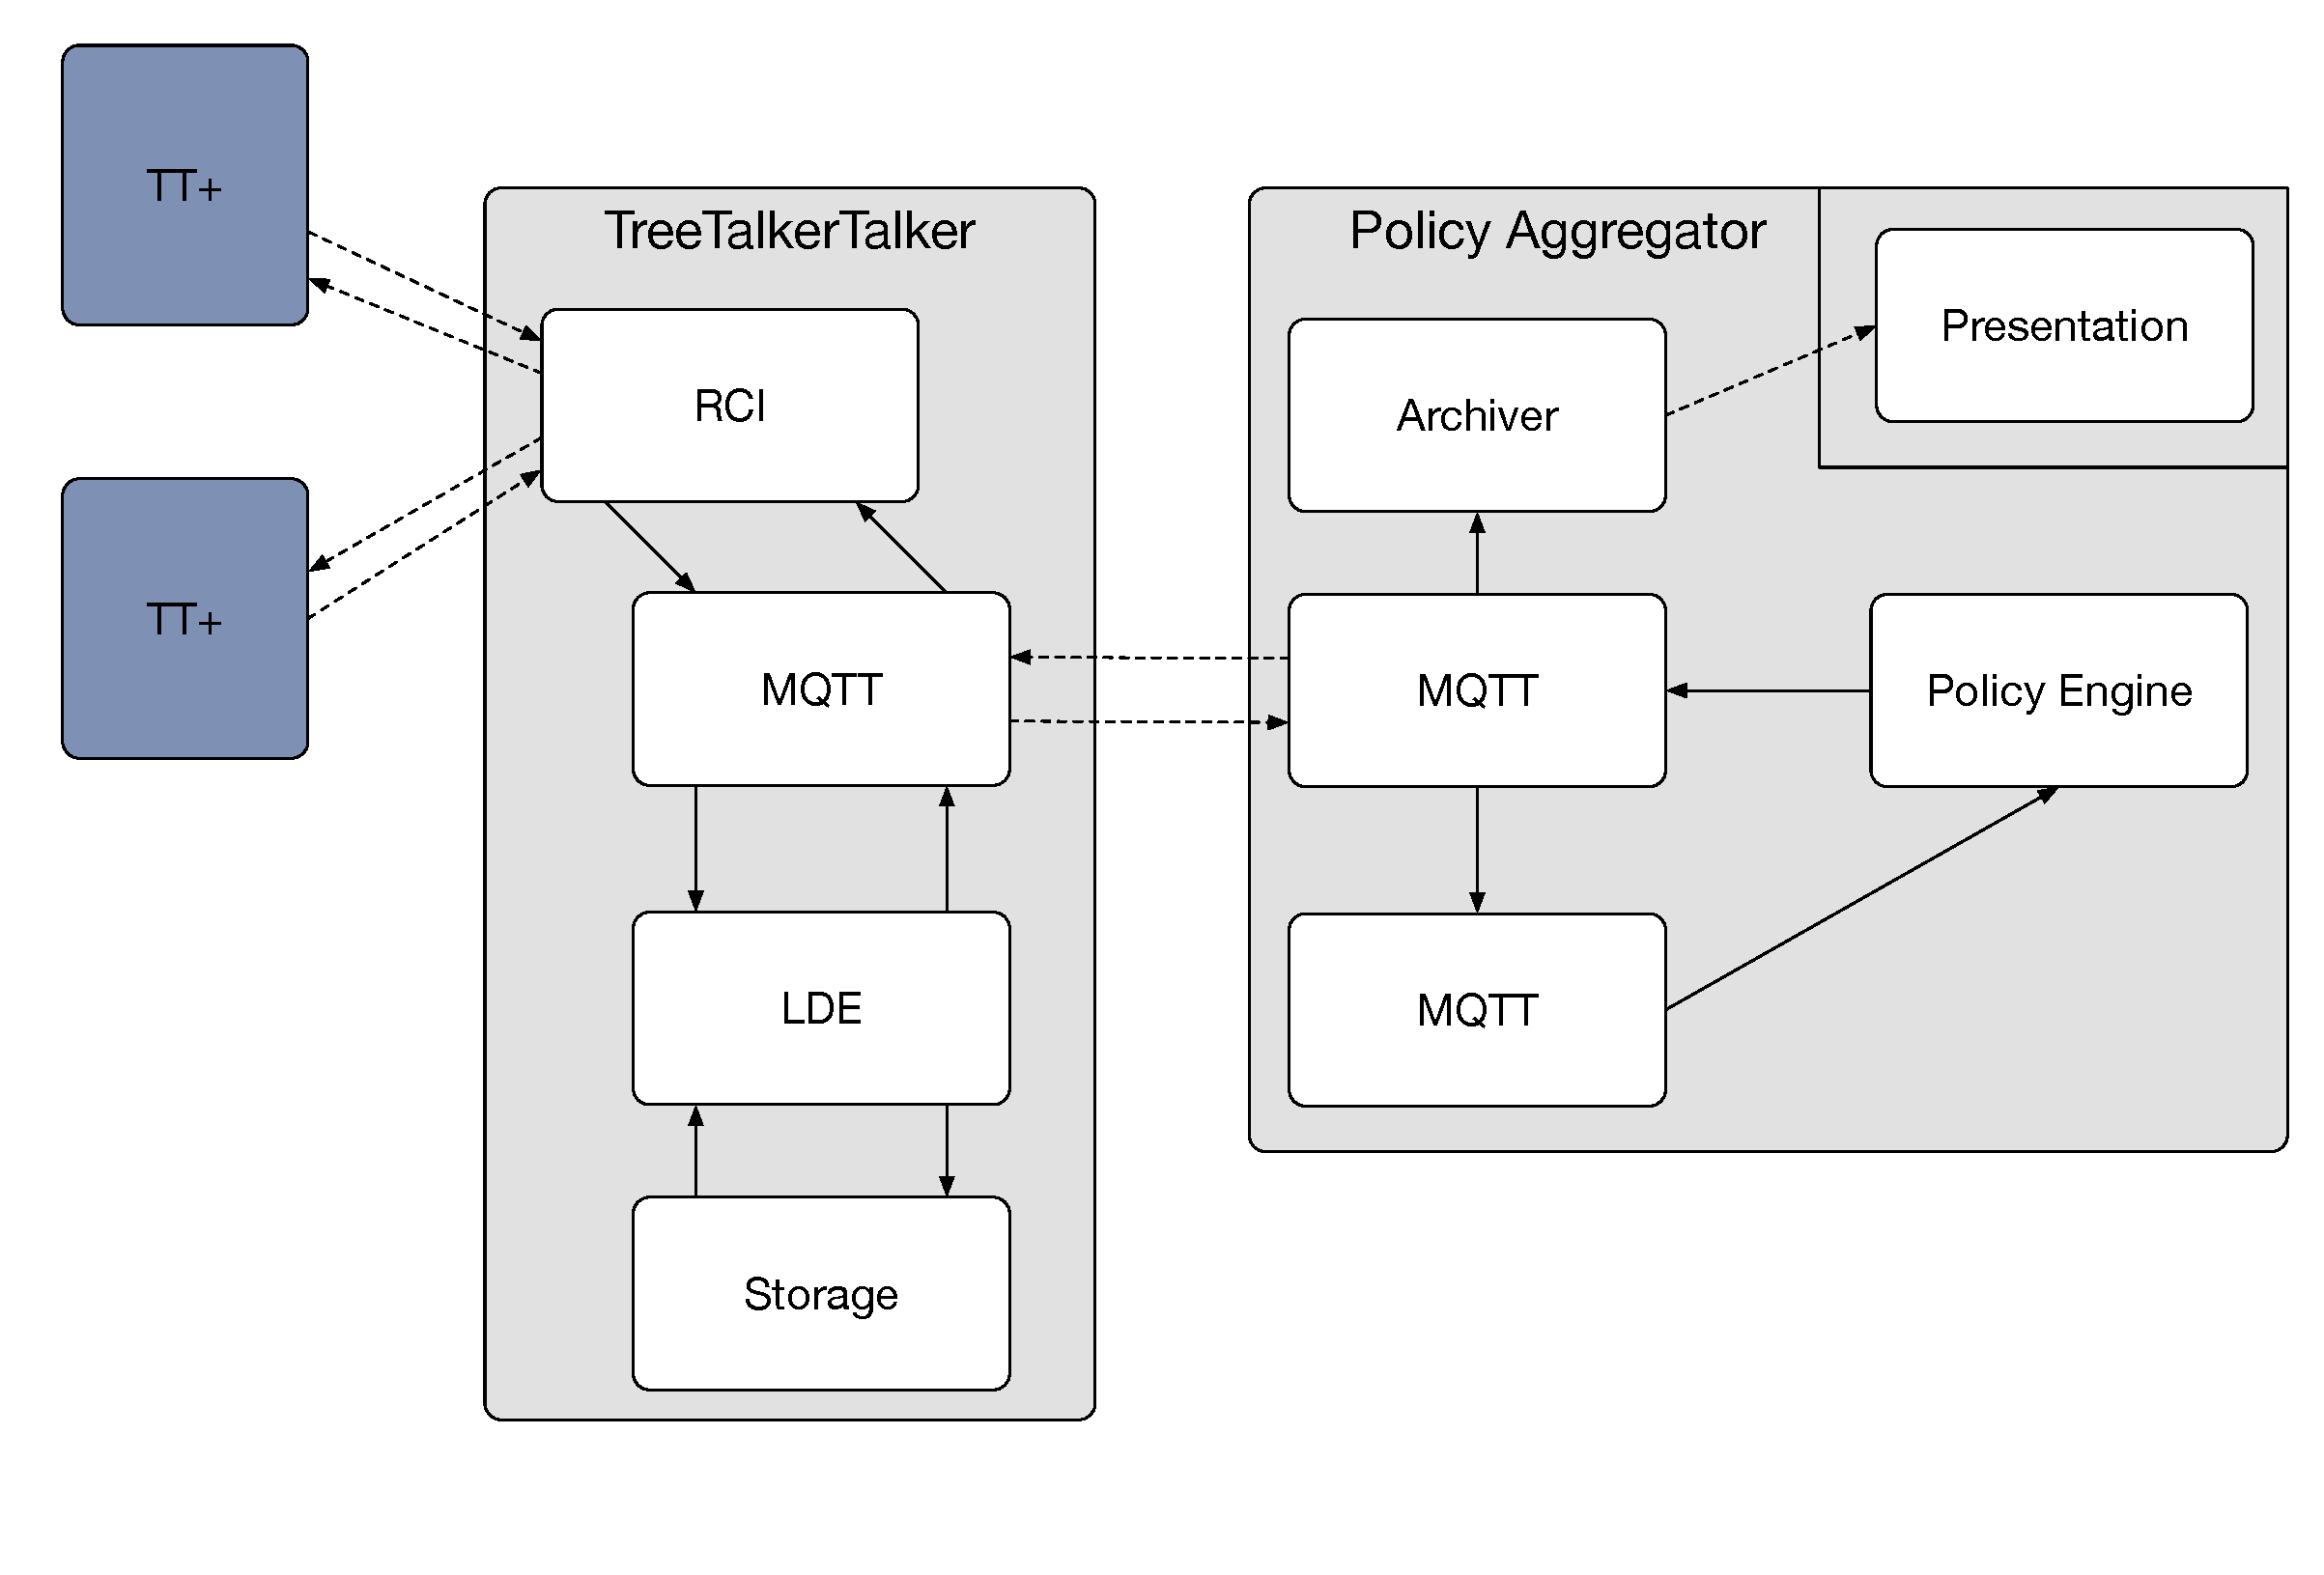
\includegraphics[width=.8\linewidth]{figures/TTT_architectur.pdf}
    \caption{System architecture of \ttt}
    \label{fig:ttt-architecture}
\end{figure}

In our implementation there are two separate decision engines. 
The local one, which is located directly on the hardware of the \textit{TreetalkerTalker} unmarshalls the received packages of individual \textit{Treetalkers} and evaluates their data packets independently of each other. 
In parallel, the local engine stores all incoming packets in a local Influx DB and forwards these packets to the cloud using the MQTT protocol. 

The values of the individual sensors are then statistically evaluated in the local decision engine. 
For this purpose, the last X \todo{Aktuelle Anzahl der betrachteten Tage einsetzen} days are averaged as a reference value. 
If individual measured values are above Y \todo{Aktueller Skalar einsetzen} times the average value, the local decision engine can initiate appropriate responses by changing the behaviour of the \textit{Treetalker}. 
The Decision Engine not only considers the immediate values but also takes other factors into account to justify a decision. 
The local decision engine is primarily used to detect anomalies on a single \textit{Treetalker}. 
Here, for example, the position sensor can be used to detect whether the \textit{Treetalker} is still correctly attached to the tree. 
Another example is the detection of a local fire using the humidity, light and temperature sensors.

In addition to the local decision engine, the system has a global decision engine that can make decisions based on the measured values of an entire \textit{Treetalker} cluster. 
For this purpose, the data from the various \textit{TreetalkerTalker} are collected in aggregate on another Influx DB on a centralized instance in the cloud and considered as a collective entity. 

The values of the global decision engine are summarized and transmitted back to the local decision engine for further processing. Based on the values from the so-called world view, the local decision engine can incorporate the data into its own calculations. In some formulas the world view can be taken over directly as a scalar into the computation, which defines thus the range of values considered as inconspicuous more exactly.

Currently, this process has to run synchronously, but in future revisions it is logical that the local decision engine only receives sporadic updates from the global decision engine and, if necessary, performs an interpolation in order to be able to run the entire process asynchronously.


One of our examples of a successful detection includes examining the motion data from the attitude sensors of an entire cluster to distinguishing a storm from a position error or a measurement/sensor error.
Another example includes looking at all available temperature sensors collectively to distinguish a fire situation from a general heat wave.


Based on these values it is possible to make more accurate decisions and to reduce the number of false positive decisions of the local decision engine and even to revise them if necessary. 
The decisions of both engines are used collectively to adjust the behavior of the \textit{Treetalkers}.

\todo{habe den folgenden Block erstmal darunter geschrieben, dieser müsste noch eingeordnet werden - an welcher Stelle macht dieser am meisten Sinn?}
In order to make decisions based on the detection, concept recognition is necessary. This is done by comparing a long-running process with a short-running one. It has been shown that the calculation of the twofold standard deviation for short-running processes is already sufficient to be able to make decisions - for example, whether a new measurement is necessary or these new values can be appointed as the new standard. In general, the preferred method for making decisions is to reduce the upcoming measurement interval in order to verify and increase the accuracy of the collected data. Due to the minor costs on battery consumption and data transmission over Lora, even 20\% double measurements are insignificant for the overall system operation. 

Administrators can be alerted on the basis of the long-running processes, provided that this reaches three times the standard deviation.

\label{sec:implementation:treetalker:error-detection}

\begin{figure}
    \centering
    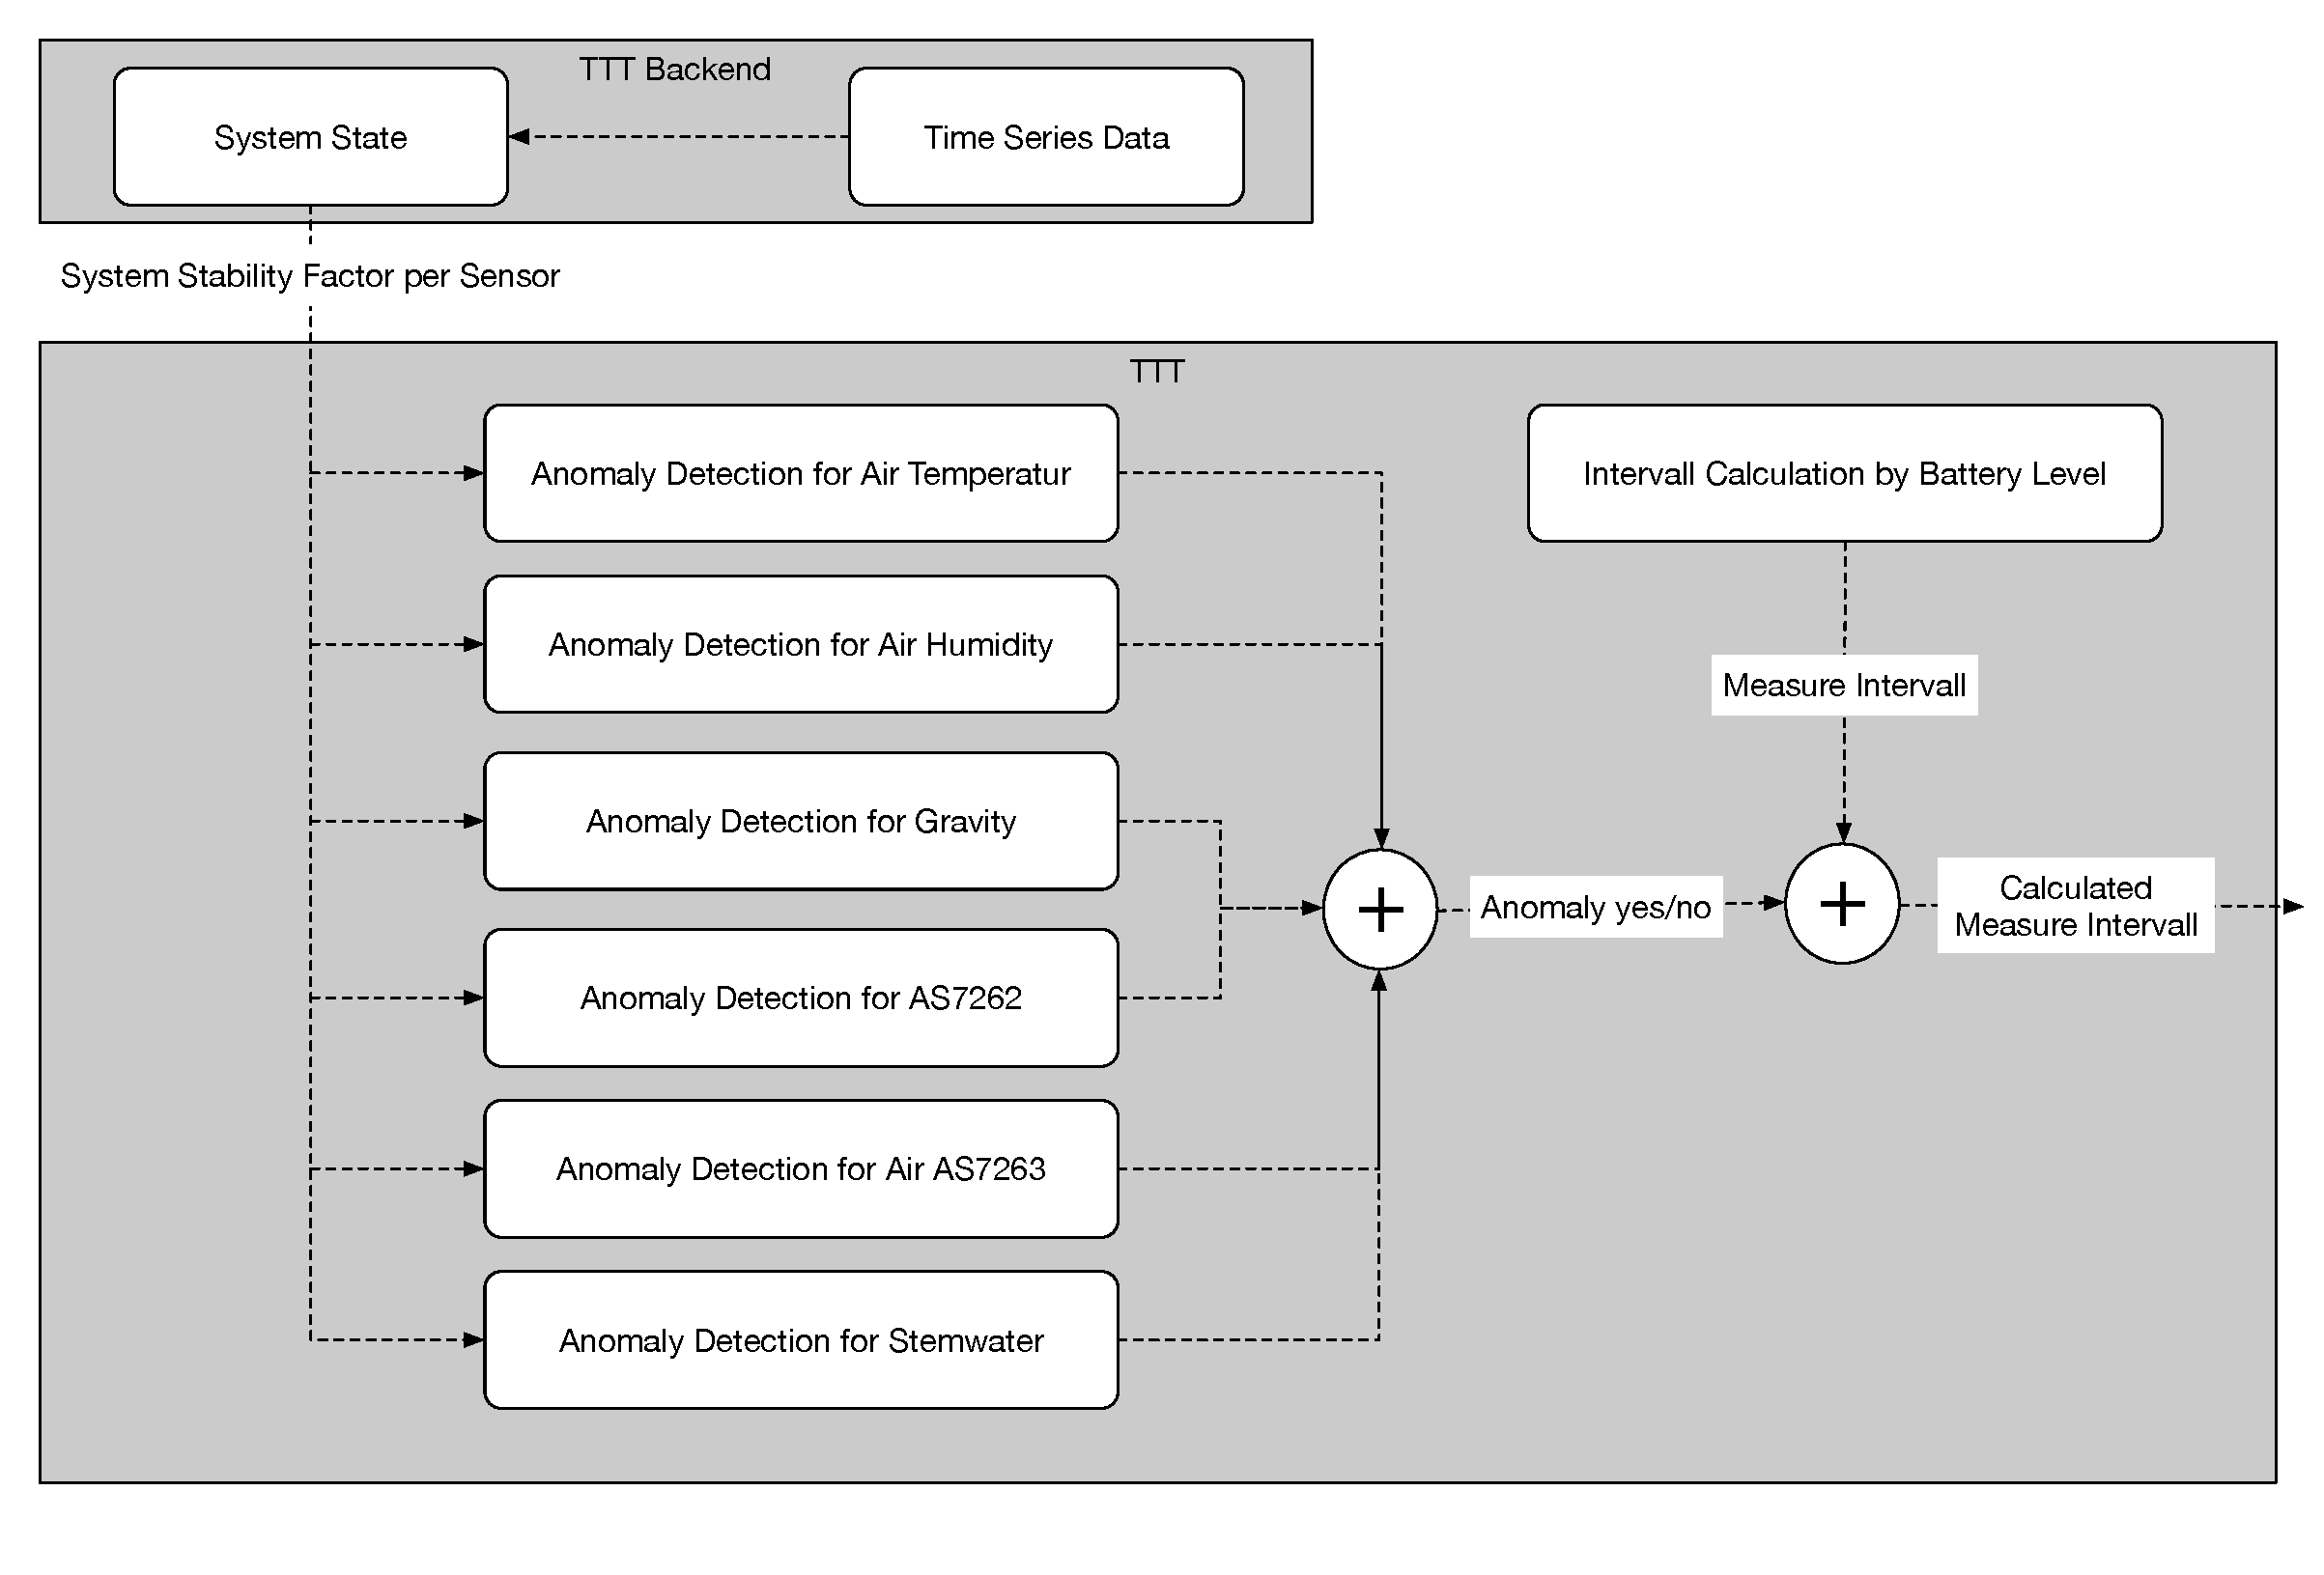
\includegraphics[width=.8\linewidth]{figures/TTT_decision_process.pdf}
    \caption{Decision process for the next measurement period for the TT+}
    \label{fig:TTT_decision_process}
\end{figure}

\subsubsection{Behavior Modification}
Based on the decisions of the two existing decision engines, it is possible to adapt the behavior of each connected \textit{Treetalker}. 
A command packet (see figures \ref{fig:ttcommand}) is expected as a response to each data packet sent by the \textit{Treetalker}. 

The command packet is used to confirm receipt of the data packet and to transmit further instructions to the \textit{Treetalker}. 
The transmission of a command packet can take a short time offset, so that the decision engine has enough available time to evaluate the data packet. 
If this packet is not received by the \textit{Treetalker}, it tries to retransmit the data packet a few times before it stores it in its local memory and tries to redo it again after a time delay. 

Depending on the type of the command packet, different settings of the \textit{Treetalker} can be overwritten and its behavior can be changed. 

For example, we are able to dynamically change both the measuring cycles and the actual measuring time of the sensors. 
If the decision engine has detected an abnormal measurement state, the measurement interval can be automatically adjusted to either reevaluate the current state and eliminate a possible measurement error as well as increase the amount of possible measurement points for further evaluation. 

To prevent the \textit{Treetalker} from entering a non-functional state, parameters such as the current state of charge of the battery are included in the calculation of the new measurement interval.
Conversely, the intervals can also be increased for certain inconspicuous measurement results in order to preserve the battery in the long term (e.g. winter mode). 

Depending on the individual decision of the decision engine, it is also possible to change the behavior of a \textit{Treetalker} based on the measurement results of the entire cloud. 
A valid use case is, for example, that all \textit{Treetalkers} in the proximity of a single \textit{Treetalker} reduce their measurement interval in the event of a spontaneously strong fluctuation of a measurement point, even if the measurement results of the individual \textit{Treetalkers} have so far been inconspicuous. 

In order to prevent congestion on the side of the radio link, it would also be possible to reduce the measurement cycle of a individual \textit{Treetalker} so that other members in the network can obtain its timeslot. 
This is particularly relevant if the number of \textit{Treetalkers} in a network exceeds 20, as this can lead to increased interference on the used frequency band, as stated by the manufacture of the \textit{Treetalkers}. \footnote{https://www.nature4shop.com/prodotto/tt-cl-modem-router-for-cloud-connection/}
This situation could also occur if third parties are active on the same frequency band and the reception of a packet could be classified as difficult in the medium term. 